\documentclass{article}
\usepackage[utf8]{inputenc}

\title{AML PA1}
\author{ajchavan }
\date{April 2017}

\usepackage{natbib}
\usepackage{graphicx}
\usepackage{lipsum}
\usepackage{mwe}

\begin{document}

\maketitle


\begin{center}
\textbf{Run program like =$>$ e.g. - python pa2\_svm.py}
\end{center}

\pagebreak

\section{Data preprocessing}

\begin{enumerate}
    \item Data preprocessing is executed in a method called preprocess\_data()
    \item Appended train and test file together and converted it to adult.csv
    \item Read csv file using pandas by speicifying na\_values=['?'] to consider for missing values and later on drop those columns using dropna() method in pandas.
    \item From the data I removed work-class race and native-country as they didn't form a substantial logic for the income prediction. After reading the data description I still didn't understand what fnlwgt meant so I looked up online and I don't think it will have any credibility for income prediction so dropped that too
    \item From the data available I found online how to convert ordinal and nominal variables to convert to boolean and feed it to sklearn estimation. For continous values too e.g. if data is in the range say different numbers from 0 to 1000 then we do the same procedure as ordinal variables  i.e. Go through entire dataset if a value corresponding to the current value is found then make it true else False. Repeat this for every unique value. Apply this same procedure for each algorithm. 
    
    I have explained this in the code too for better understanding.
    
    
    \item Since we are predicting whether income is greater than \$50K or not I use $>$ \$50K as the parameter and drop $<$= \$50K
    
\end{enumerate}

\pagebreak

\section{Training the data}

\begin{enumerate}
    \item After the procedure for preprocessing data we train the data for the 4 Machine Learning algorithms
    \item In training I split train/test to 0.8/0.2.
    \item Using sklearn fit the X and y from the training data from preprocessing data and then predict using Xtest and ytest
    \item Using classification\_report from sklearn.metrics we get precision recall and f1 score and support.
    \item After that using predict\_proba for the given estimator to get the yscore and getting roc value using it.
    
\end{enumerate}
 
\pagebreak

\section{Choice of parameter = ROC}

I chose ROC as a better performance measure as opposed to F1 score Precision Recall because of 2 reasons:

1. Data is not askewed. Every attribute of a given category isn't equally distributed and so accuracy cannot be considered as a reliable measure 

2. Our main aim is to maximize our prediction(TPR) or minimize the error. This can be best measured by using ROC curve by finding the ratio of True Positive rate vs False Positive Rate. So even though precision and recall are good measures but for current case ROC works the best.

\pagebreak

\section{ Effect of Hyperparameters}

%Logisitc reg less tol = better perf
%Decisoin tree = less tree prob more tree prob 10 perf
%nb = binarize = 0 = good 1 = bad

\subsection{SVM}

For SVM more the value of C better the result. 

Below is output for C=0.1,0.5,1.0:   

\begin{figure}
    \centering
    \begin{minipage}{0.45\textwidth}
        \centering
        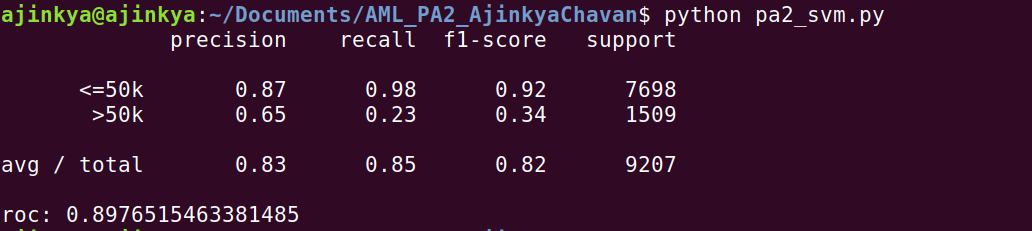
\includegraphics[width=0.9\textwidth]{svm_01.png} %  itself
        \caption{svm C=0.1}
    \end{minipage}\hfill
    \begin{minipage}{0.45\textwidth}
        \centering
        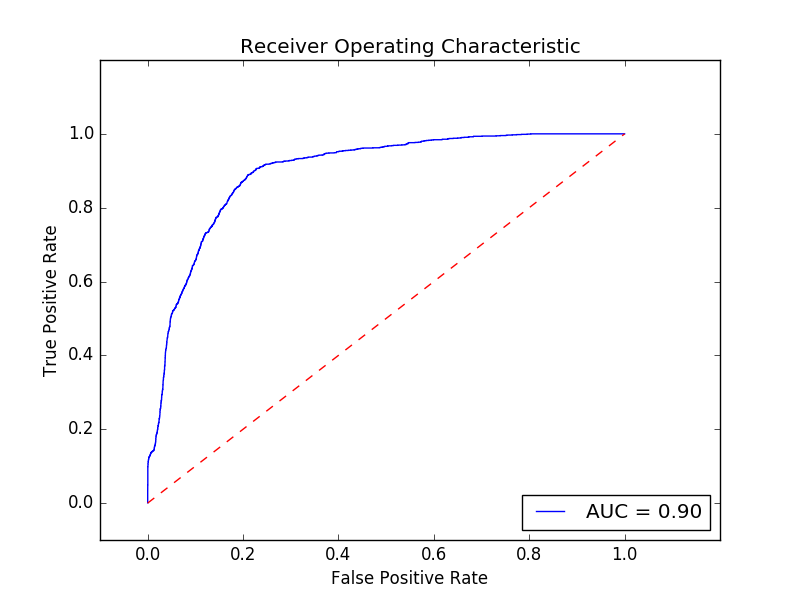
\includegraphics[width=0.9\textwidth]{roc_svm_01.png} %  itself
        \caption{svm roc C=0.1}
    \end{minipage}
\end{figure}

\begin{figure}
    \centering
    \begin{minipage}{0.45\textwidth}
        \centering
        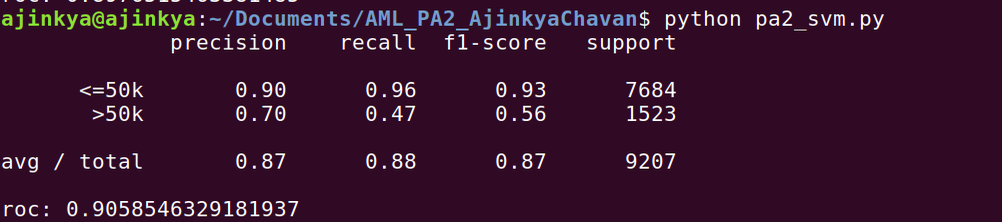
\includegraphics[width=0.9\textwidth]{svm_05.png} %  itself
        \caption{svm C=0.5}
    \end{minipage}\hfill
    \begin{minipage}{0.45\textwidth}
        \centering
        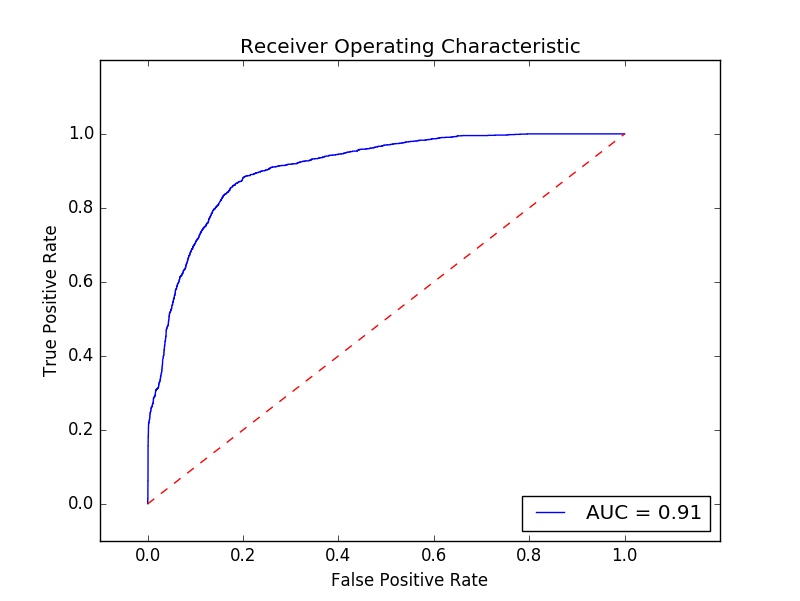
\includegraphics[width=0.9\textwidth]{roc_svm_05.png} %  itself
        \caption{svm roc C=0.5}
    \end{minipage}
\end{figure}

\begin{figure}
    \centering
    \begin{minipage}{0.45\textwidth}
        \centering
        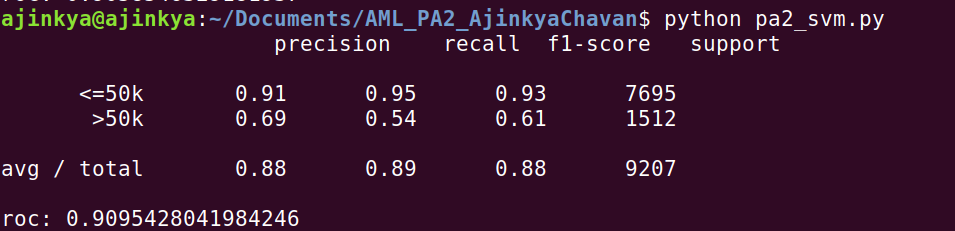
\includegraphics[width=0.9\textwidth]{svm_10.png} %  itself
        \caption{svm C=1.0}
    \end{minipage}\hfill
    \begin{minipage}{0.45\textwidth}
        \centering
        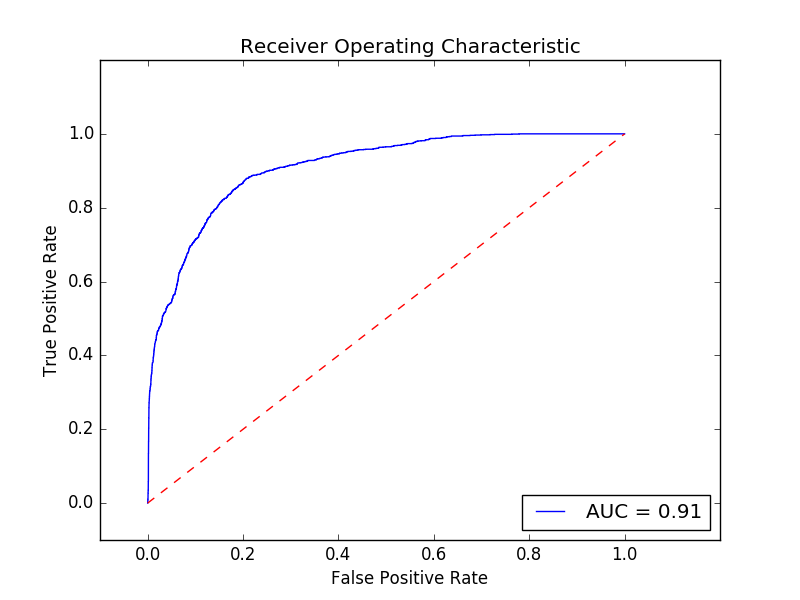
\includegraphics[width=0.9\textwidth]{roc_svm_10.png} %  itself
        \caption{svm roc C=1.0}
    \end{minipage}
\end{figure}



\subsection{Random Forest}

In random forest as the number of estimators grow the accuracy increases till a point where we find a perfect combination of number of estimators and max\_depth. After that point the accuracy decreases again however the decrease in accuracy is not as steep for a given number of estimators with higher depths. 

Below is the output for number of estimators and depth combinations of : (5,5)(5,50)(5,100)(50,5)(50,50)(50,100)(100,5)(100,50)(100,100)






\begin{figure}
    \centering
    \begin{minipage}{0.45\textwidth}
        \centering
        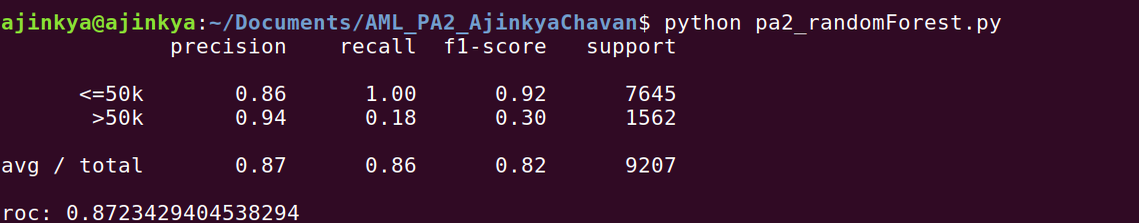
\includegraphics[width=0.9\textwidth]{random_5_5.png} %  itself
        \caption{random forest estimators=5  depth=5}
    \end{minipage}\hfill
    \begin{minipage}{0.45\textwidth}
        \centering
        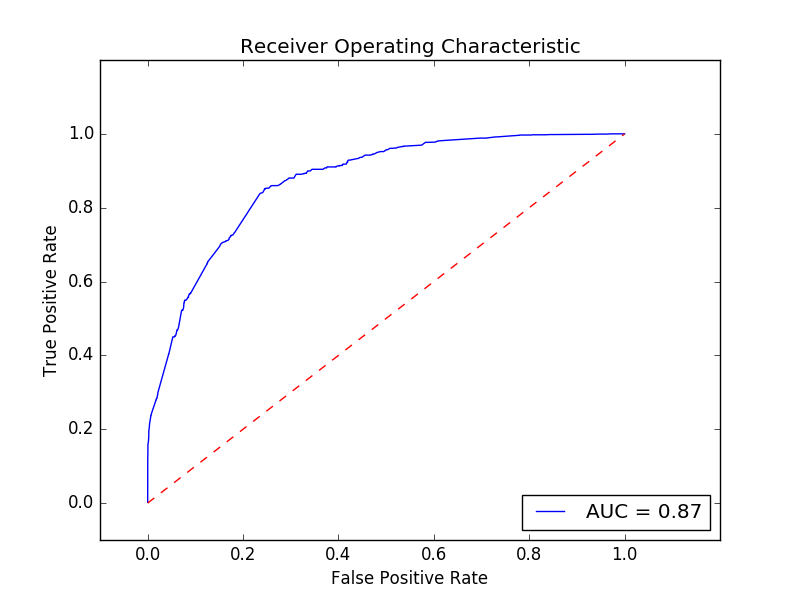
\includegraphics[width=0.9\textwidth]{roc_random_5_5.png} %  itself
        \caption{random forest roc estimators=5 depth=5}
    \end{minipage}
\end{figure}




\begin{figure}
    \centering
    \begin{minipage}{0.45\textwidth}
        \centering
        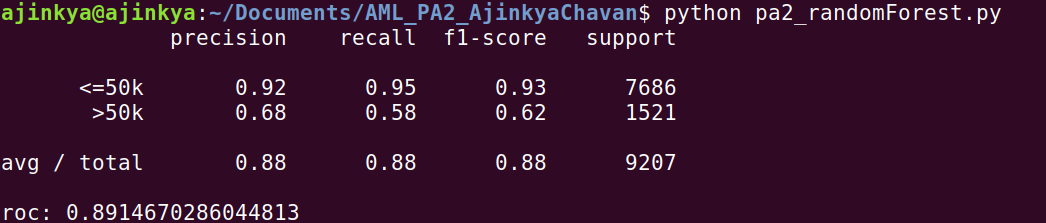
\includegraphics[width=0.9\textwidth]{random_5_50.png} %  itself
        \caption{random forest estimators=5 depth=50}
    \end{minipage}\hfill
    \begin{minipage}{0.45\textwidth}
        \centering
        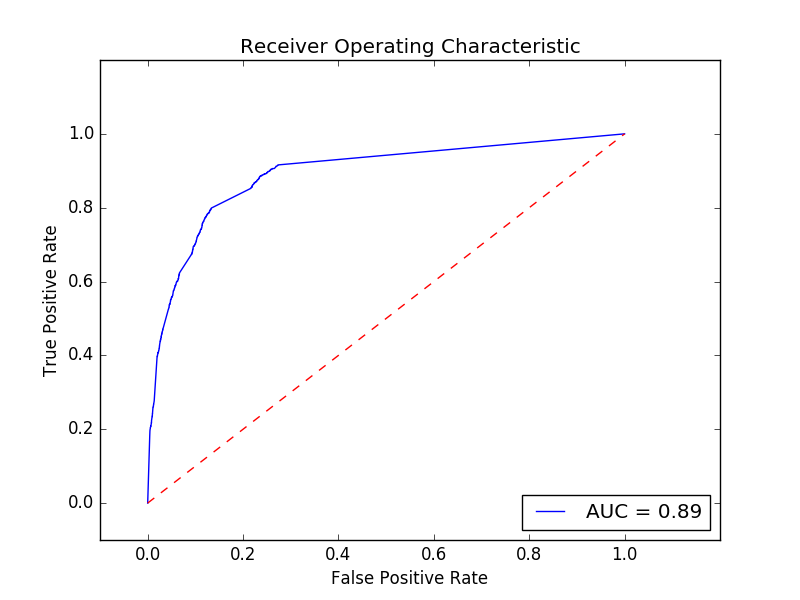
\includegraphics[width=0.9\textwidth]{roc_random_5_50.png} %  itself
        \caption{random forest roc estimators=5 depth=50}
    \end{minipage}
\end{figure}






\begin{figure}
    \centering
    \begin{minipage}{0.45\textwidth}
        \centering
        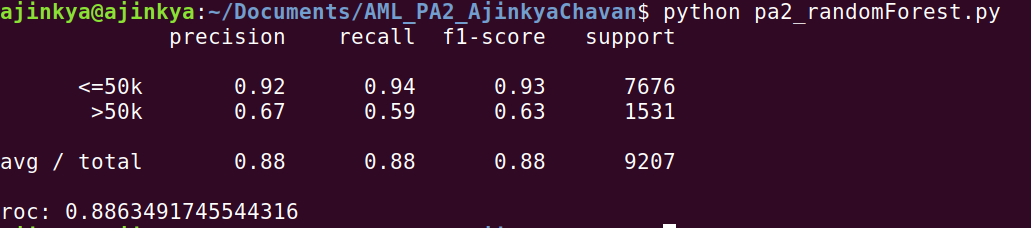
\includegraphics[width=0.9\textwidth]{random_5_100.png} %  itself
        \caption{random forest estimators=5 depth=100}
    \end{minipage}\hfill
    \begin{minipage}{0.45\textwidth}
        \centering
        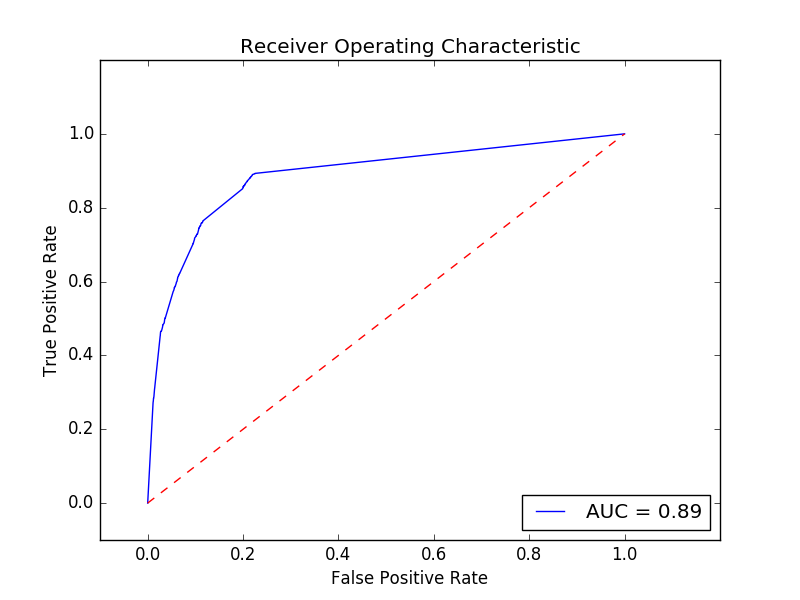
\includegraphics[width=0.9\textwidth]{roc_random_5_100.png} %  itself
        \caption{roc random forest estimators=5 depth=100}
    \end{minipage}
\end{figure}







\begin{figure}
    \centering
    \begin{minipage}{0.45\textwidth}
        \centering
        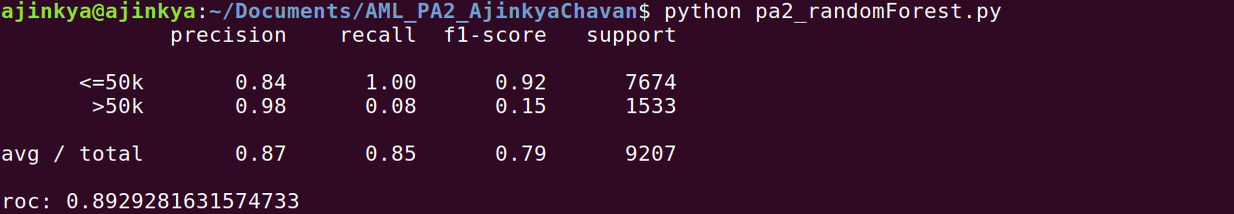
\includegraphics[width=0.9\textwidth]{random_50_5.png} %  itself
        \caption{random forest estimators=50 depth=5}
    \end{minipage}\hfill
    \begin{minipage}{0.45\textwidth}
        \centering
        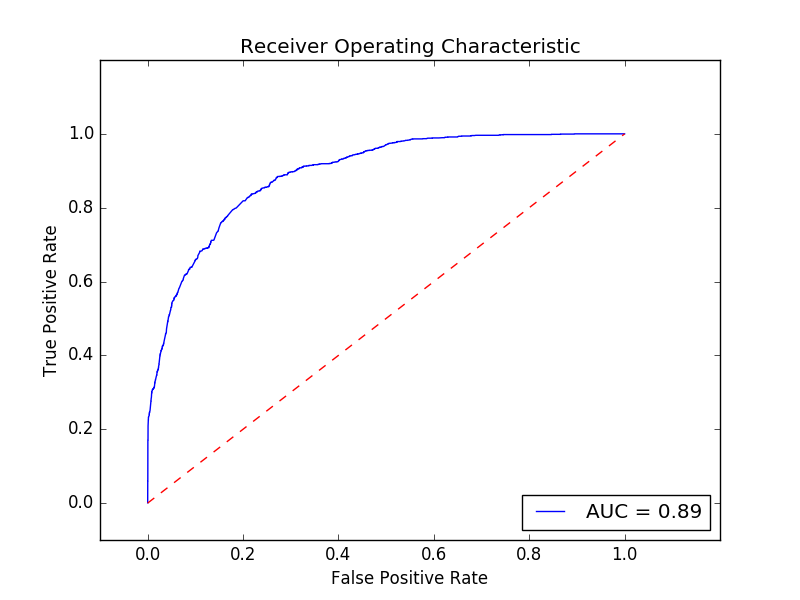
\includegraphics[width=0.9\textwidth]{roc_random_50_5.png} %  itself
        \caption{roc random forest estimators=50 depth=5}
    \end{minipage}
\end{figure}







\begin{figure}
    \centering
    \begin{minipage}{0.45\textwidth}
        \centering
        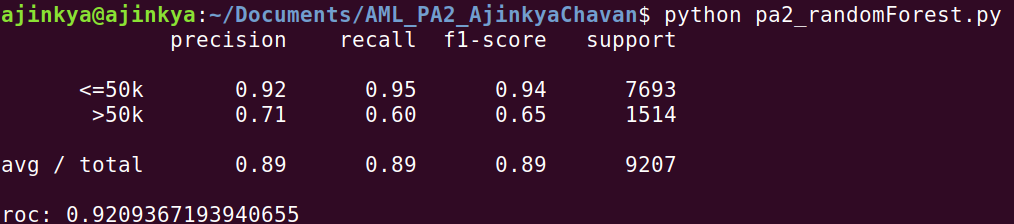
\includegraphics[width=0.9\textwidth]{random_50_50.png} %  itself
        \caption{random forest estimators=50 depth=50}
    \end{minipage}\hfill
    \begin{minipage}{0.45\textwidth}
        \centering
        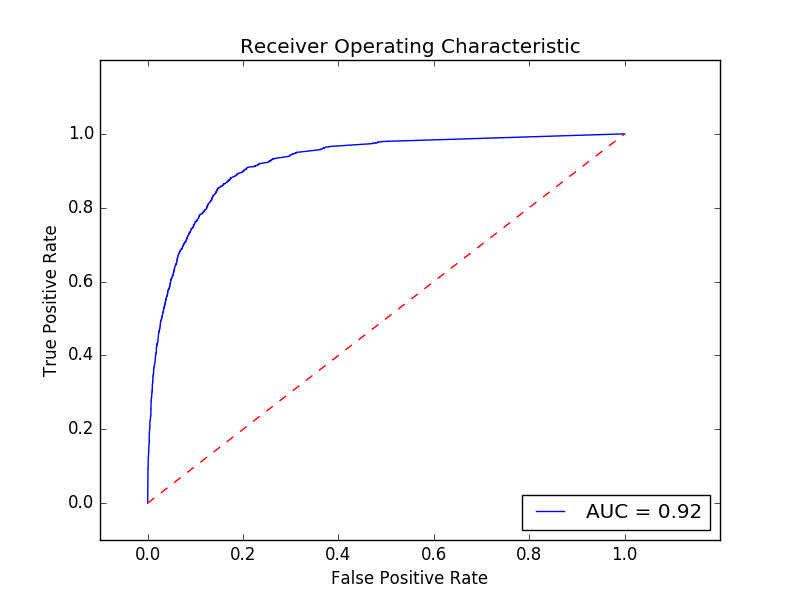
\includegraphics[width=0.9\textwidth]{roc_random_50_50.png} %  itself
        \caption{roc random forest estimators=50 depth=50}
    \end{minipage}
\end{figure}






\begin{figure}
    \centering
    \begin{minipage}{0.45\textwidth}
        \centering
        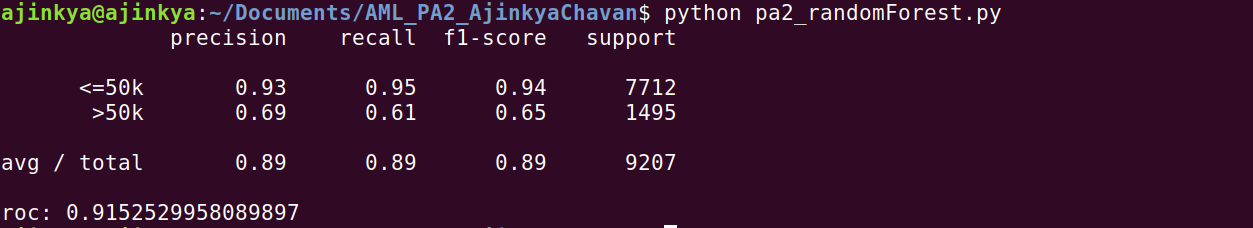
\includegraphics[width=0.9\textwidth]{random_50_100.png} %  itself
        \caption{random forest estimators=50 depth=100}
    \end{minipage}\hfill
    \begin{minipage}{0.45\textwidth}
        \centering
        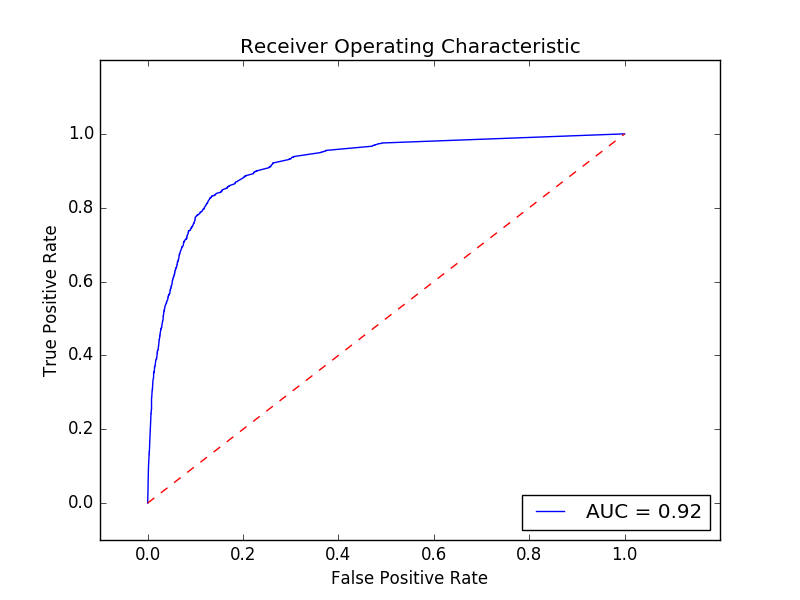
\includegraphics[width=0.9\textwidth]{roc_random_50_100.png} %  itself
        \caption{roc random forest estimators=50 depth=100}
    \end{minipage}
\end{figure}






\begin{figure}
    \centering
    \begin{minipage}{0.45\textwidth}
        \centering
        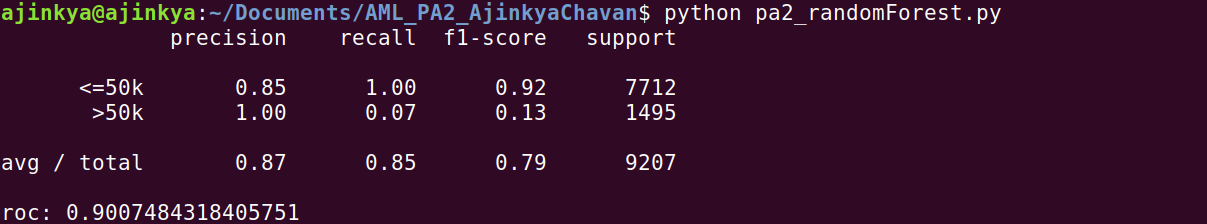
\includegraphics[width=0.9\textwidth]{random_100_5.png} %  itself
        \caption{random forest estimators=100 depth=5}
    \end{minipage}\hfill
    \begin{minipage}{0.45\textwidth}
        \centering
        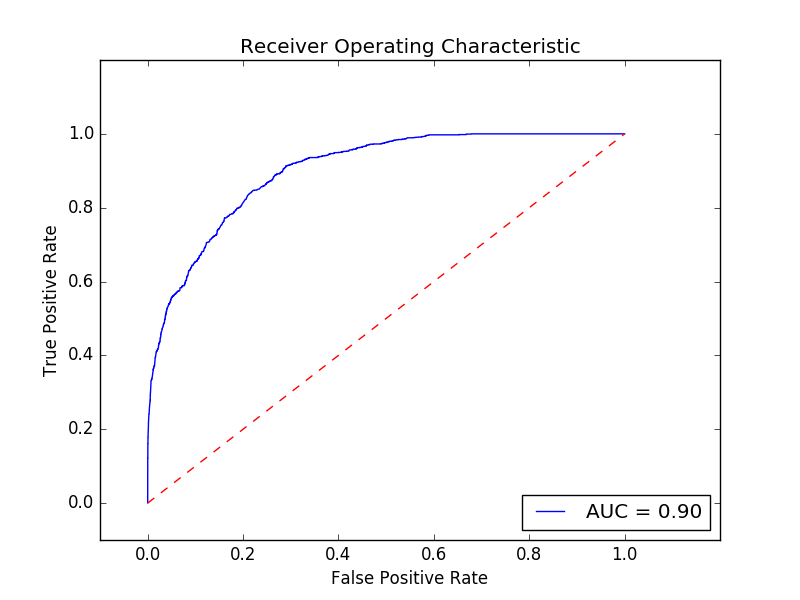
\includegraphics[width=0.9\textwidth]{roc_random_100_5.png} %  itself
        \caption{roc random forest estimators=100 depth=5}
    \end{minipage}
\end{figure}







\begin{figure}
    \centering
    \begin{minipage}{0.45\textwidth}
        \centering
        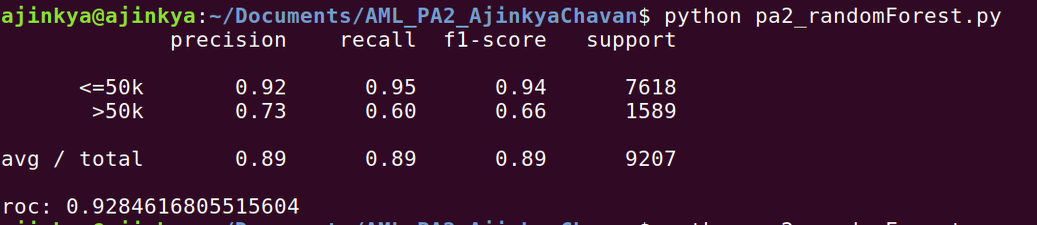
\includegraphics[width=0.9\textwidth]{random_100_50.png} %  itself
        \caption{random forest estimators=100 depth=50}
    \end{minipage}\hfill
    \begin{minipage}{0.45\textwidth}
        \centering
        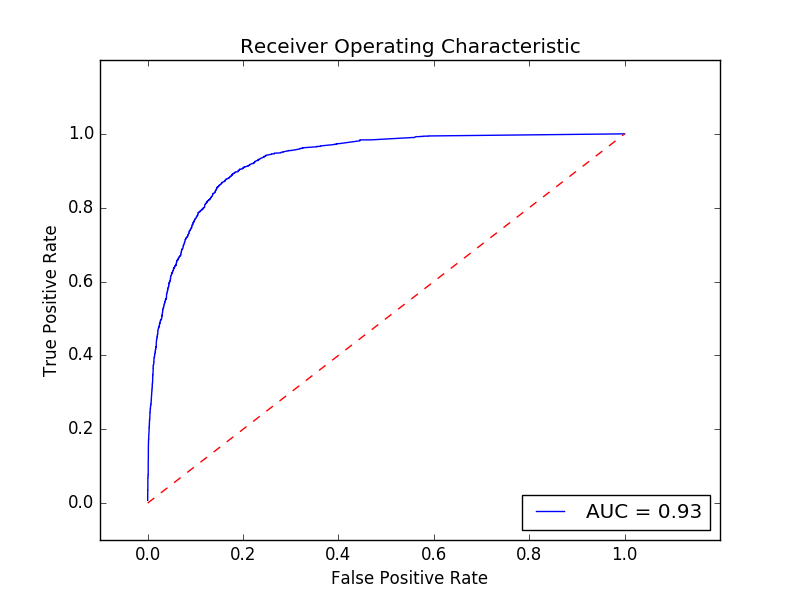
\includegraphics[width=0.9\textwidth]{roc_random_100_50.png} %  itself
        \caption{roc random forest estimators=100 depth=50}
    \end{minipage}
\end{figure}





\begin{figure}
    \centering
    \begin{minipage}{0.45\textwidth}
        \centering
        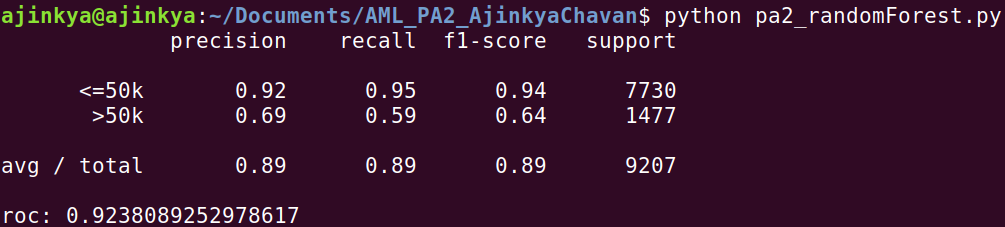
\includegraphics[width=0.9\textwidth]{random_100_100.png} %  itself
        \caption{random forest estimators=100 depth=100}
    \end{minipage}\hfill
    \begin{minipage}{0.45\textwidth}
        \centering
        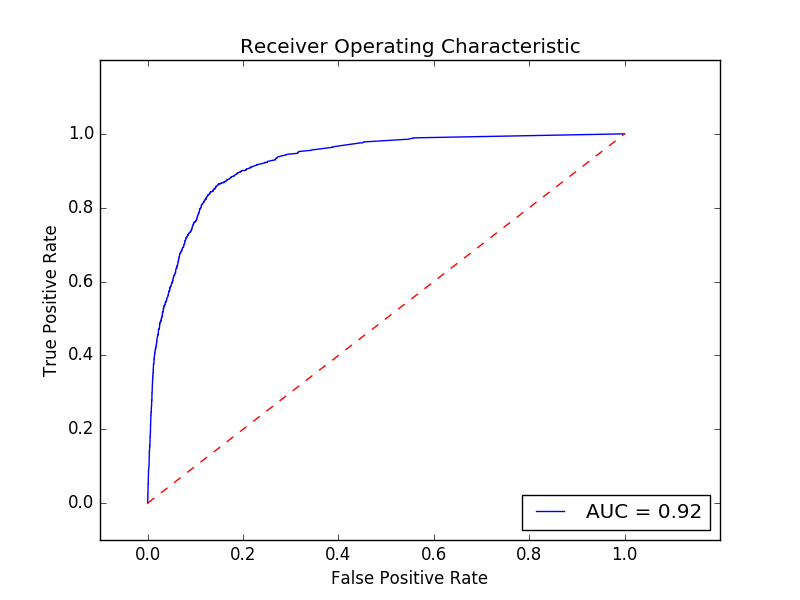
\includegraphics[width=0.9\textwidth]{roc_random_100_100.png} %  itself
        \caption{roc random forest estimators=100 depth=100}
    \end{minipage}
\end{figure}

\pagebreak 
\pagebreak

\subsection{Adaboost}

I used Decision tree as the base estimator for Adaboost. From the combinations of number of estimators and depth of the tree I found that for number of estimators =5 50 100 -> lesser the depth of tree better the results. As depth increases the accuracy decreases beyond a certain point of combination of number of estimators and depth. 


Below is the output for number of estimators and depth combinations of : for:(5,5)(5,50)(5,100)(50,5)(50,50)(50,100)(100,5)(100,50)(100,100)


\begin{figure}
    \centering
    \begin{minipage}{0.45\textwidth}
        \centering
        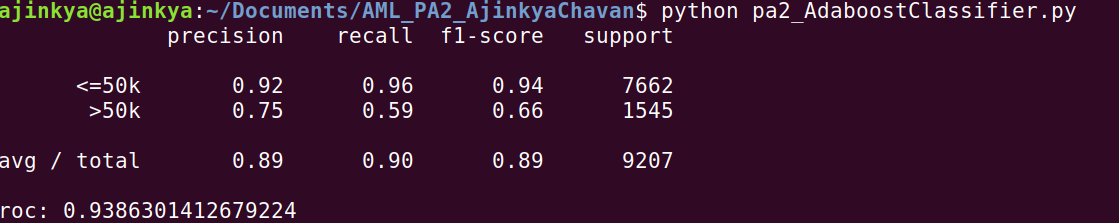
\includegraphics[width=0.9\textwidth]{ada_5_5.png} %  itself
        \caption{ada estimators=5 depth=5}
    \end{minipage}\hfill
    \begin{minipage}{0.45\textwidth}
        \centering
        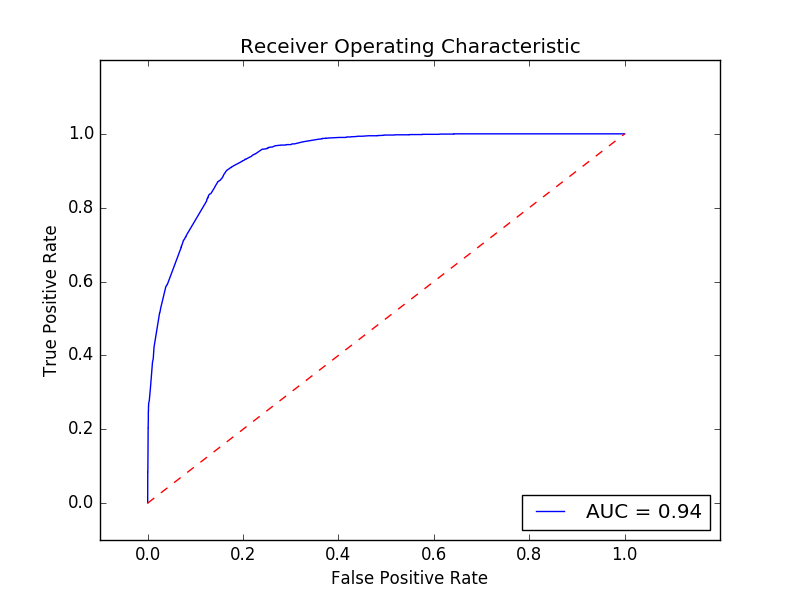
\includegraphics[width=0.9\textwidth]{roc_ada_5_5.png} %  itself
        \caption{roc ada estimators=5 depth=5}
    \end{minipage}
\end{figure}








\begin{figure}
    \centering
    \begin{minipage}{0.45\textwidth}
        \centering
        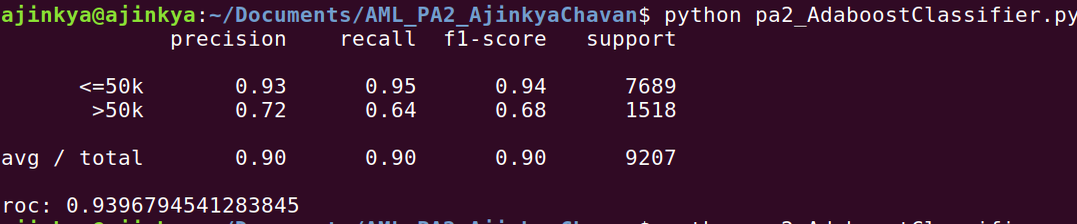
\includegraphics[width=0.9\textwidth]{ada_5_50.png} %  itself
        \caption{ada estimators=5 depth=50}
    \end{minipage}\hfill
    \begin{minipage}{0.45\textwidth}
        \centering
        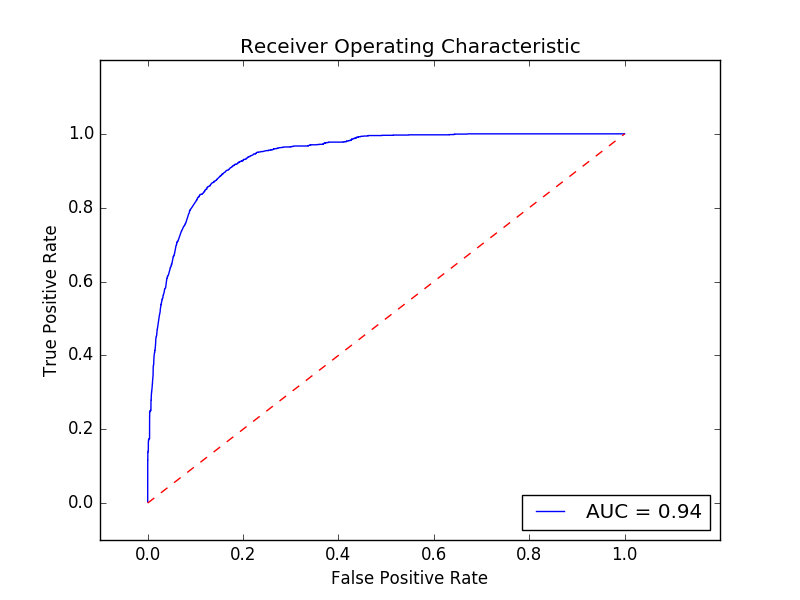
\includegraphics[width=0.9\textwidth]{roc_ada_5_50.png} %  itself
        \caption{roc ada estimators=5 depth=50}
    \end{minipage}
\end{figure}






\begin{figure}
    \centering
    \begin{minipage}{0.45\textwidth}
        \centering
        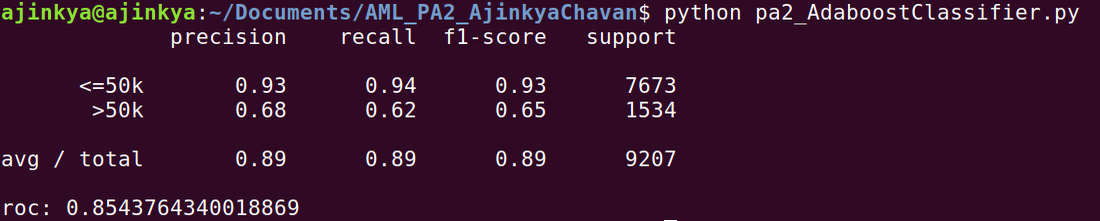
\includegraphics[width=0.9\textwidth]{ada_5_100.png} %  itself
        \caption{ada estimators=5 depth=100}
    \end{minipage}\hfill
    \begin{minipage}{0.45\textwidth}
        \centering
        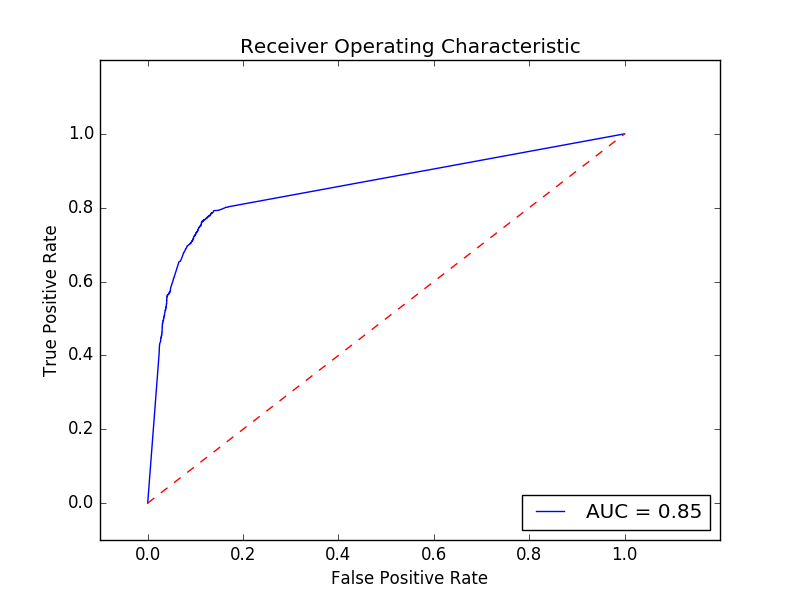
\includegraphics[width=0.9\textwidth]{roc_ada_5_100.png} %  itself
        \caption{roc ada estimators=5 depth=100}
    \end{minipage}
\end{figure}







\begin{figure}
    \centering
    \begin{minipage}{0.45\textwidth}
        \centering
        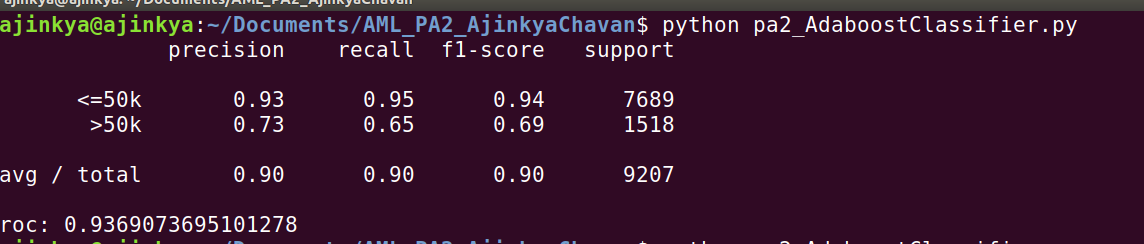
\includegraphics[width=0.9\textwidth]{ada_50_5.png} %  itself
        \caption{ada estimators=50 depth=5}
    \end{minipage}\hfill
    \begin{minipage}{0.45\textwidth}
        \centering
        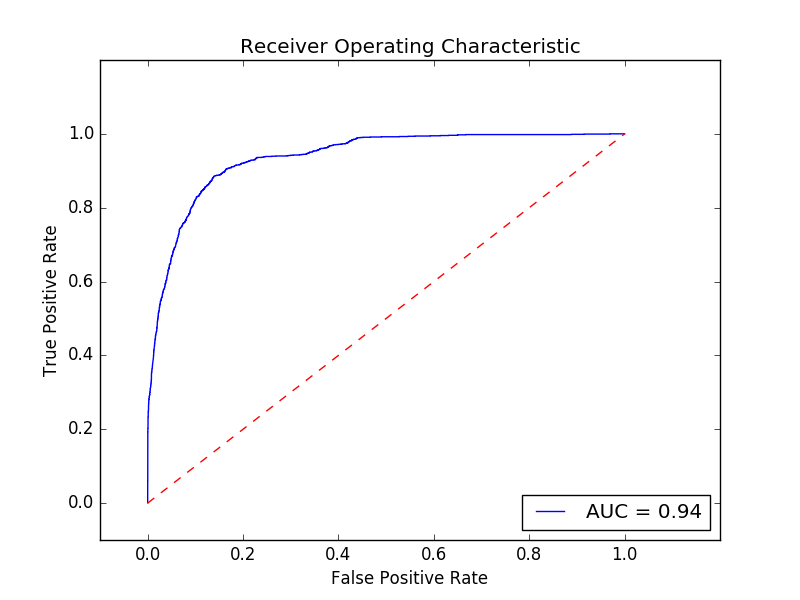
\includegraphics[width=0.9\textwidth]{roc_ada_50_5.png} %  itself
        \caption{roc ada estimators=50 depth=5}
    \end{minipage}
\end{figure}







\begin{figure}
    \centering
    \begin{minipage}{0.45\textwidth}
        \centering
        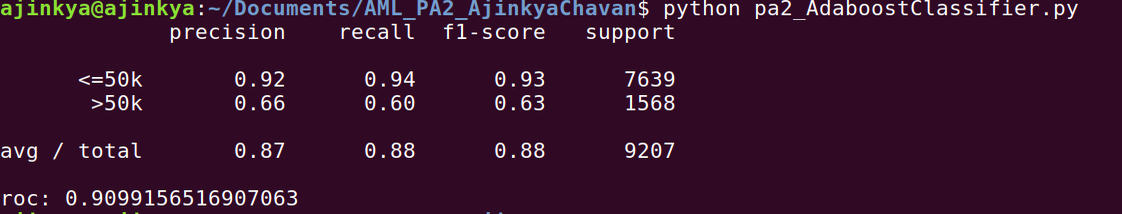
\includegraphics[width=0.9\textwidth]{ada_50_50.png} %  itself
        \caption{ada estimators=50 depth=50}
    \end{minipage}\hfill
    \begin{minipage}{0.45\textwidth}
        \centering
        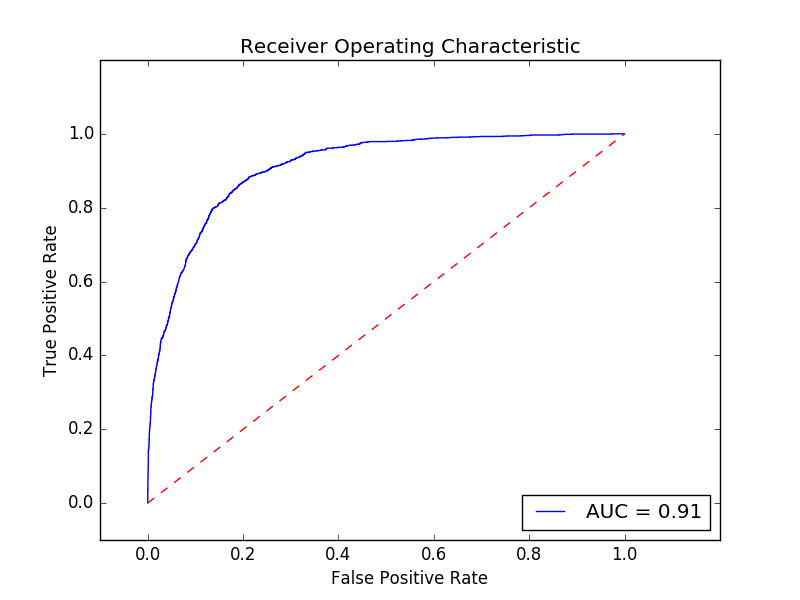
\includegraphics[width=0.9\textwidth]{roc_ada_50_50.png} %  itself
        \caption{roc ada estimators=50 depth=50}
    \end{minipage}
\end{figure}






\begin{figure}
    \centering
    \begin{minipage}{0.45\textwidth}
        \centering
        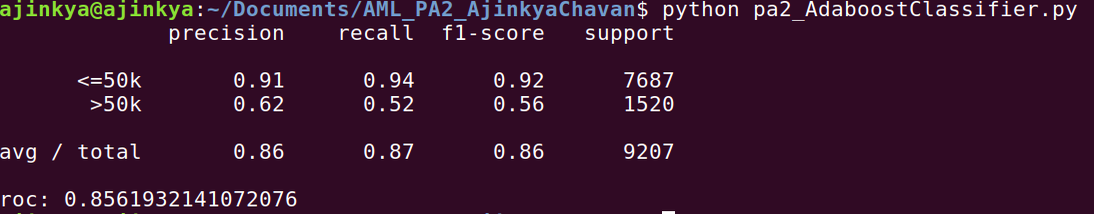
\includegraphics[width=0.9\textwidth]{ada_50_100.png} %  itself
        \caption{ada estimators=50 depth=100}
    \end{minipage}\hfill
    \begin{minipage}{0.45\textwidth}
        \centering
        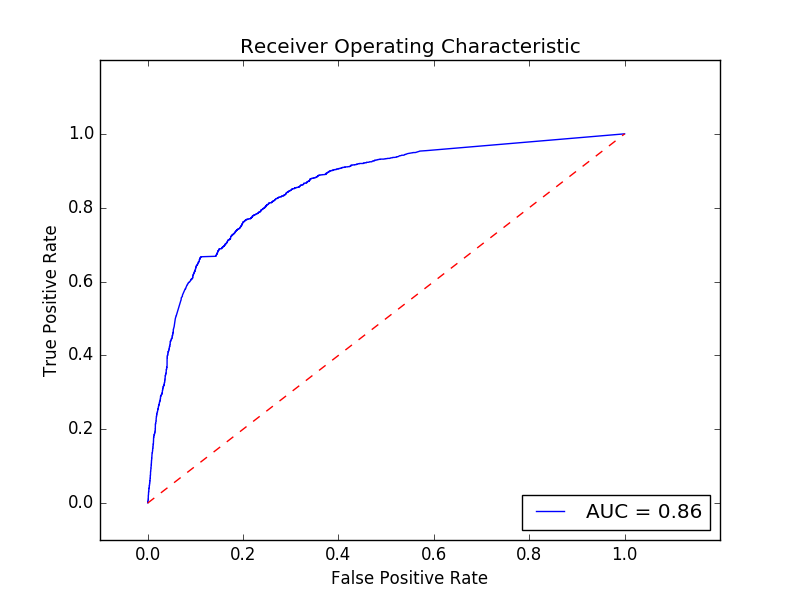
\includegraphics[width=0.9\textwidth]{roc_ada_50_100.png} %  itself
        \caption{roc ada estimators=50 depth=100}
    \end{minipage}
\end{figure}






\begin{figure}
    \centering
    \begin{minipage}{0.45\textwidth}
        \centering
        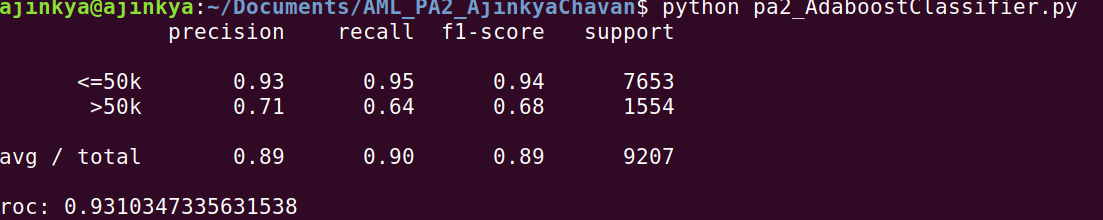
\includegraphics[width=0.9\textwidth]{ada_100_5.png} %  itself
        \caption{ada estimators=100 depth=5}
    \end{minipage}\hfill
    \begin{minipage}{0.45\textwidth}
        \centering
        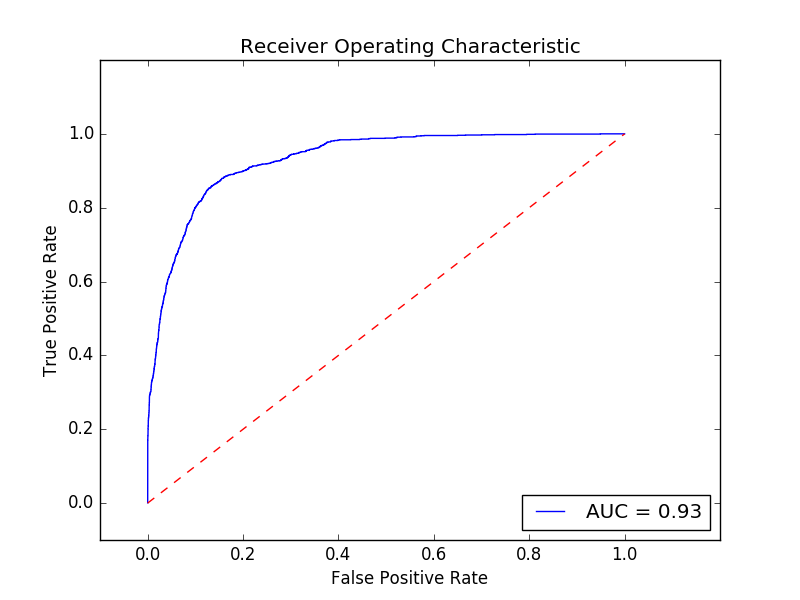
\includegraphics[width=0.9\textwidth]{roc_ada_100_5.png} %  itself
        \caption{roc ada estimators=100 depth=5}
    \end{minipage}
\end{figure}







\begin{figure}
    \centering
    \begin{minipage}{0.45\textwidth}
        \centering
        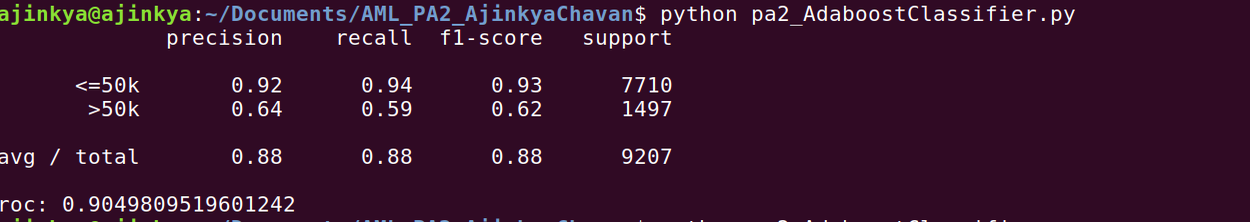
\includegraphics[width=0.9\textwidth]{ada_100_50.png} %  itself
        \caption{ada estimators=100 depth=50}
    \end{minipage}\hfill
    \begin{minipage}{0.45\textwidth}
        \centering
        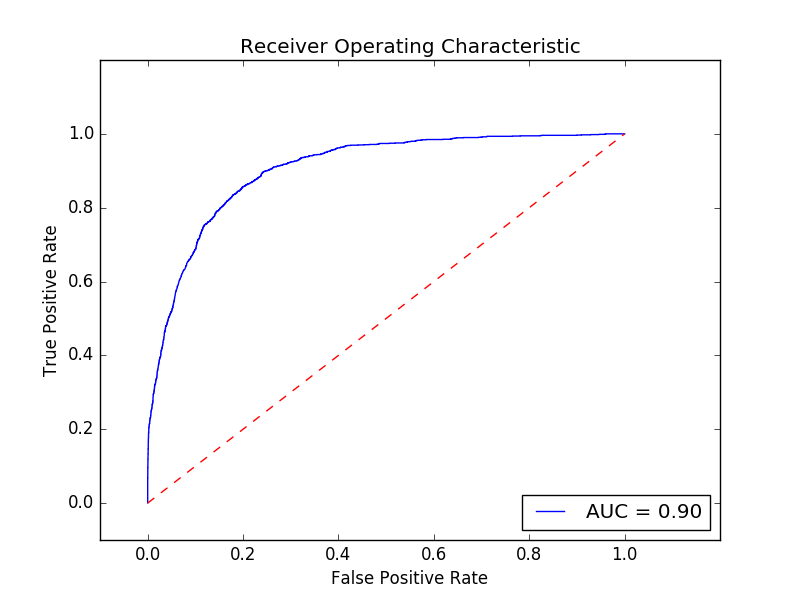
\includegraphics[width=0.9\textwidth]{roc_ada_100_50.png} %  itself
        \caption{roc ada estimators=100 depth=50}
    \end{minipage}
\end{figure}





\begin{figure}
    \centering
    \begin{minipage}{0.45\textwidth}
        \centering
        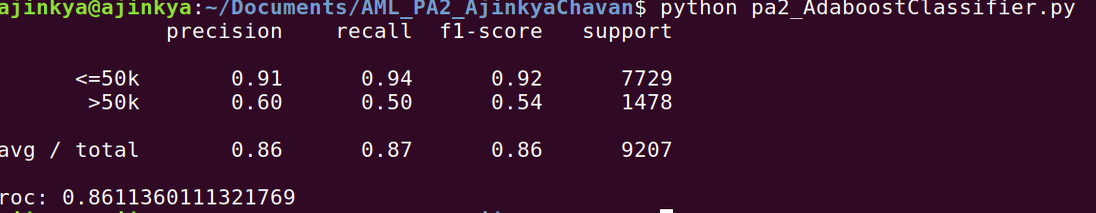
\includegraphics[width=0.9\textwidth]{ada_100_100.png} %  itself
        \caption{ada estimators=100 depth=100}
    \end{minipage}\hfill
    \begin{minipage}{0.45\textwidth}
        \centering
        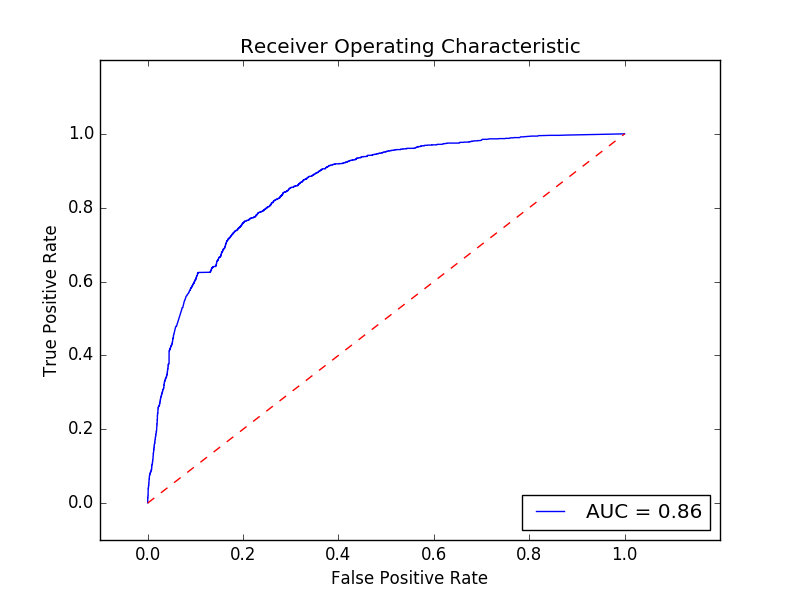
\includegraphics[width=0.9\textwidth]{roc_ada_100_100.png} %  itself
        \caption{roc ada estimators=100 depth=100}
    \end{minipage}
\end{figure}


\pagebreak
    



\section{Performance comparison}

SVM is non-parametric model and hence training gets more expensive with larger datasets.

The complex and larger dataset leads to more number of support vectors and lots of tuning is required in SVM, where as in Random forest and Adaboost, its not adherent to a lot of tuning and is worry-free approach. So SVM's are not the best choice as compared to Random Forest and Adaboost.

Between Random forest and Adaboost, we could think of Random forest as more of a bagging technique. In random forests, there are parallel ensembles, i.e. each model is built independently and its aim is to decrease variance. So random  forests are very good for high variance low bias models.

While Adaboost is as the name goes, a boosting technique. Its aim is to decrease bias and works great with high bias low variance models. 

So if we have to speak about their performance comparison, the best answer would be I think a combination of Random forests and Adaboot i.e bagging and boosting to lower variance and bias to get a good result.



Random Forest \approx  Adaboaost > SVM 

\end{document}
